% ----------------------------------------------------------------------

\newpage

\subsection{\alivetest Test}
\label{ss:alive}

\subsubsection{Purpose}

Once the pretest is completed, we can be relatively sure that all non-faulty pixels should respond to the calibration pulse.
The \alivetest test uses this fact to identify faulty pixels.
Because a pixel can be faulty in multiple ways, this test flags three types of defective pixels:
dead pixels, unmaskable pixels, and pixels with addressing errors.

\subsubsection{Methodology}

In the {\tt Alive} test, a number of calibration pulses (default 10) are sent, in turn,
to each pixel in the device and the number of signals recorded is measured.
During this period, all pixels other than the one being tested are masked, so as not to produce spurious noise signals.
Pixels with no recorded hits are flagged as dead and pixels with less than 100\% efficiency are flagged as problematic.
\\\\
In the {\tt Mask} test, all pixels are disabled and the same procedure is performed.
Pixels with efficiency above zero have a problem with the pixel masking procedure, and are flagged as bad.
\\\\
In the {\tt AddressDecoding} test, the same efficiency measurement is performed, pixel by pixel,
but the order of the resulting data is checked.
If the address of a given pixel is out of order, the recorded hit is given a negative pulse height value.
Pixels with negative hits are flagged as faulty.
\\\\
To distinguish between dead pixels and otherwise faulty pixels in output of the {\tt Mask} and {\tt AddressDecoding} tests, 
a special 3-state color scheme is used:  
Entries with a weight of 1 denote good pixels,
entries with a weight of 0 denote dead but not faulty pixels,
and entries with a weight of -1 denote faulty pixels, i.e. masking (decoding) errors for the {\tt Mask} ({\tt AddressDecoding}) test.
Figures~\ref{fig:alive_PixelAlive}-\ref{fig:alive_AddressDecodingTest} show the output from the \alivetest test.

\subsubsection{Output}

\begin{figure}[!Hp]
\centering
\begin{minipage}{0.45\textwidth}
  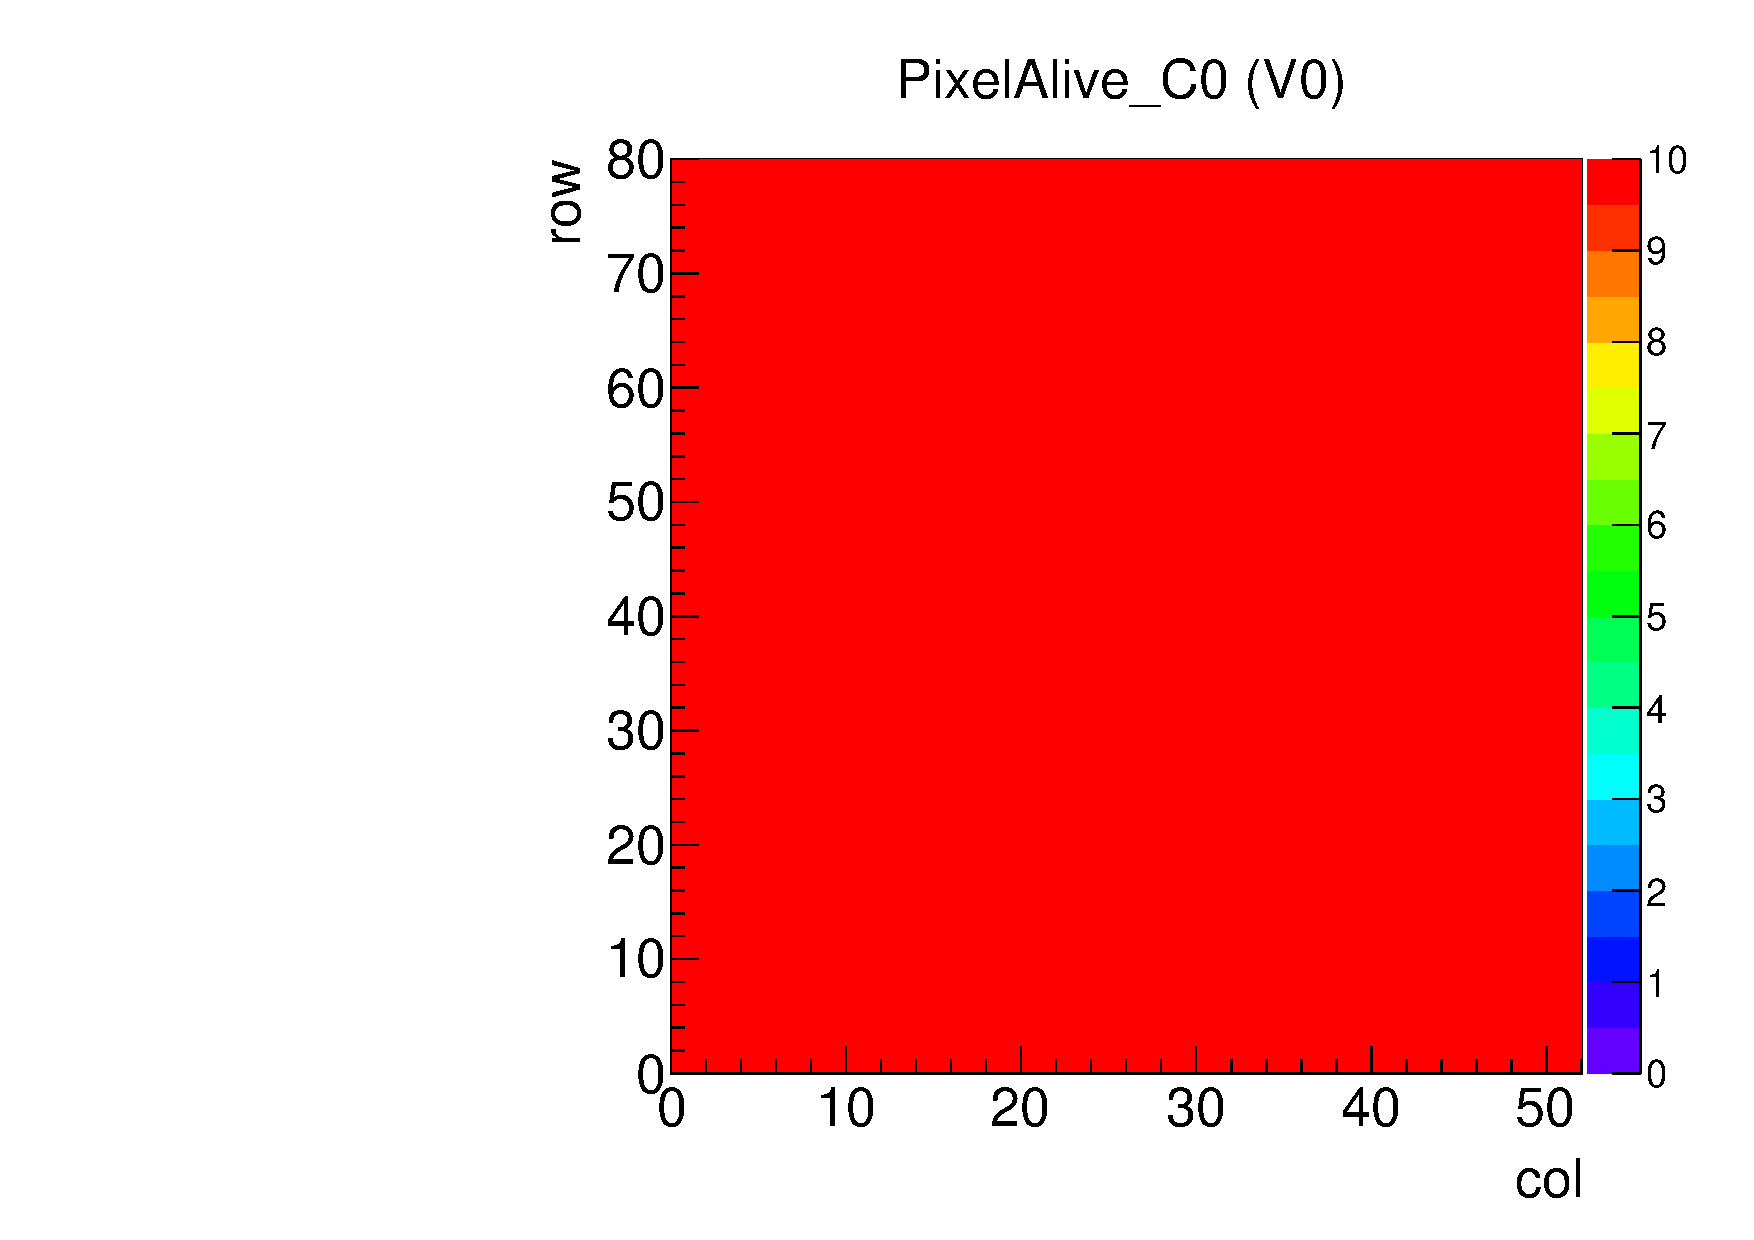
\includegraphics[width=1.0\textwidth]{figures/alive_PixelAlive.pdf}
  \caption{Created by the {\tt Alive} test. 
  Efficiency corresponds to bin content divided by number of triggers (here 10).}
  \label{fig:alive_PixelAlive}
\end{minipage}
\hspace{0.3cm}
\begin{minipage}{0.45\textwidth}
  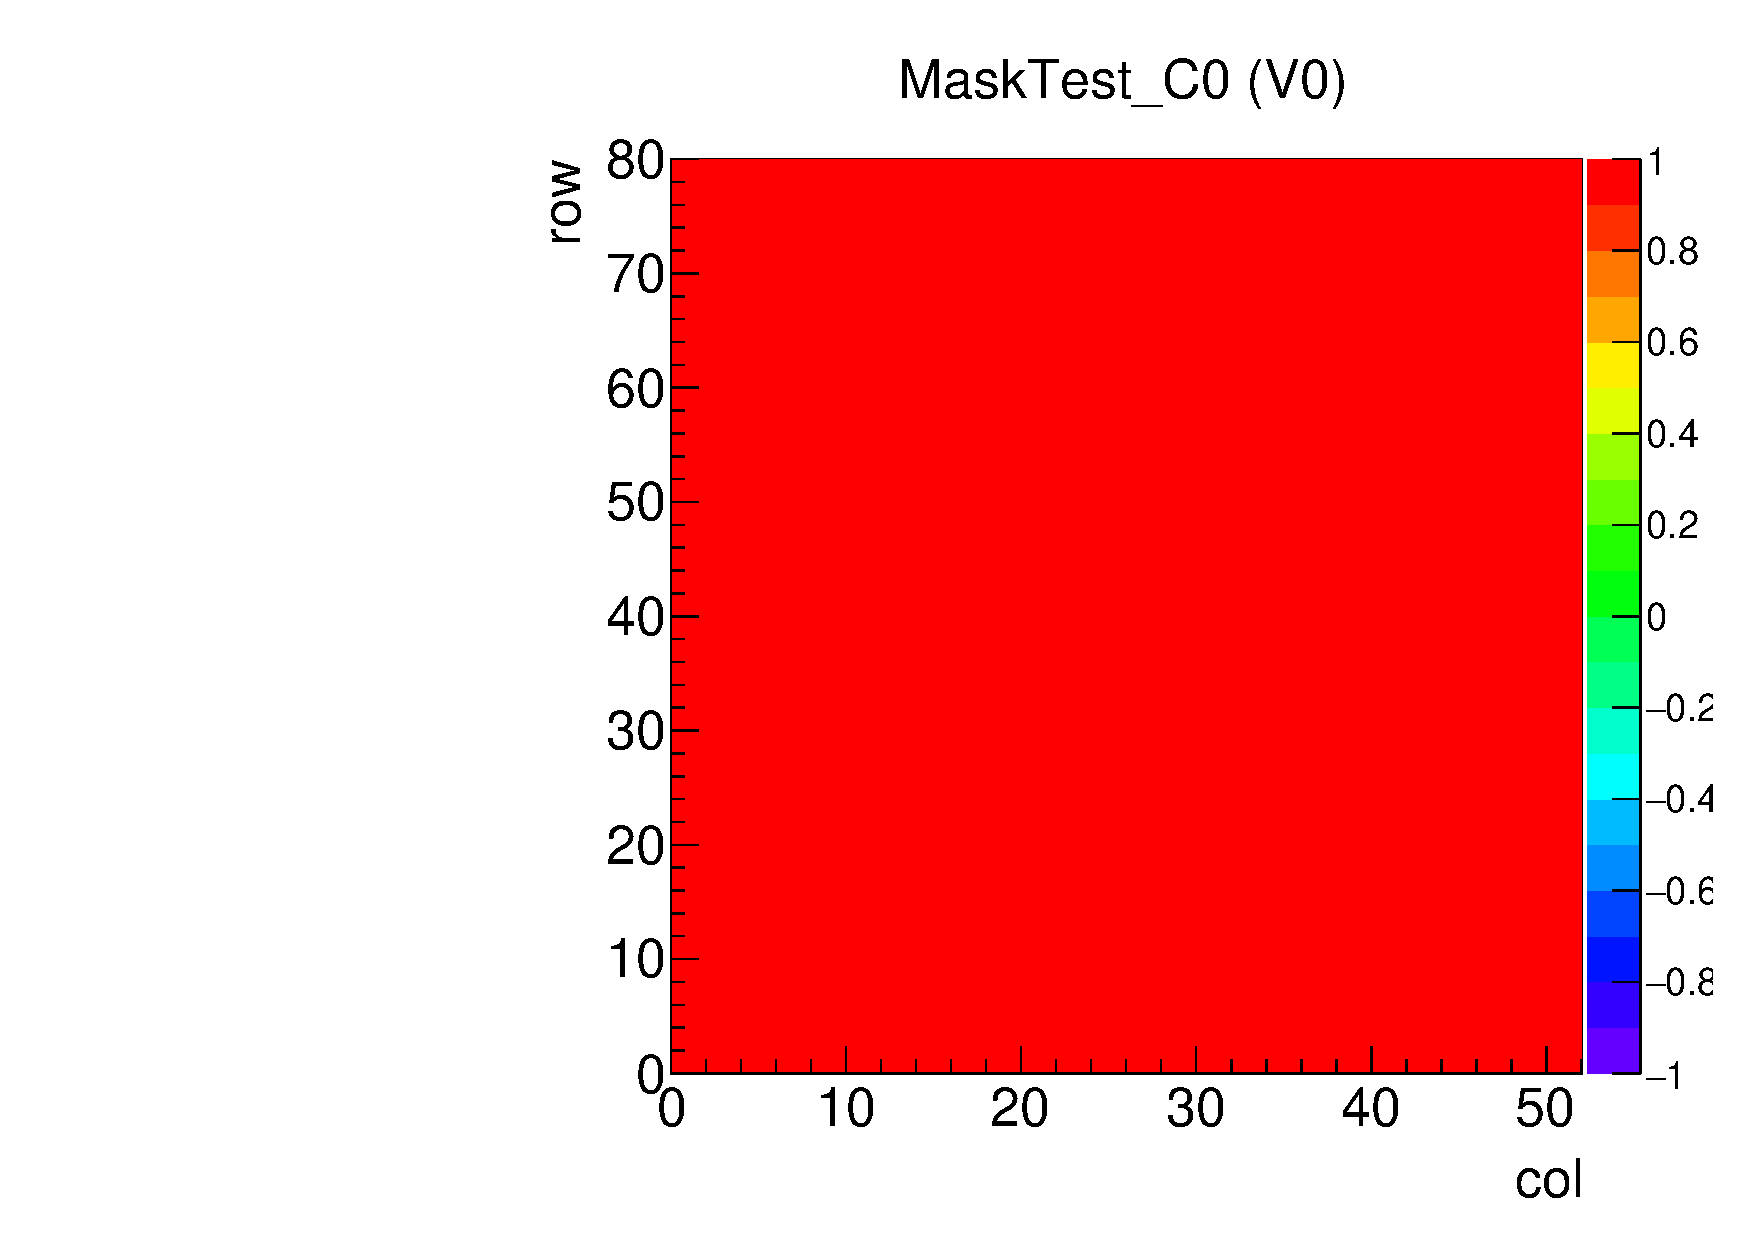
\includegraphics[width=1.0\textwidth]{figures/alive_MaskTest.pdf}
  \caption{Created by the {\tt Mask} test.
  1 (good), 0 (dead), -1 (mask problem).}
  \label{fig:alive_MaskTest}
\end{minipage}
\end{figure}

\begin{figure}[!Hp]
\centering
\begin{minipage}{0.45\textwidth}
  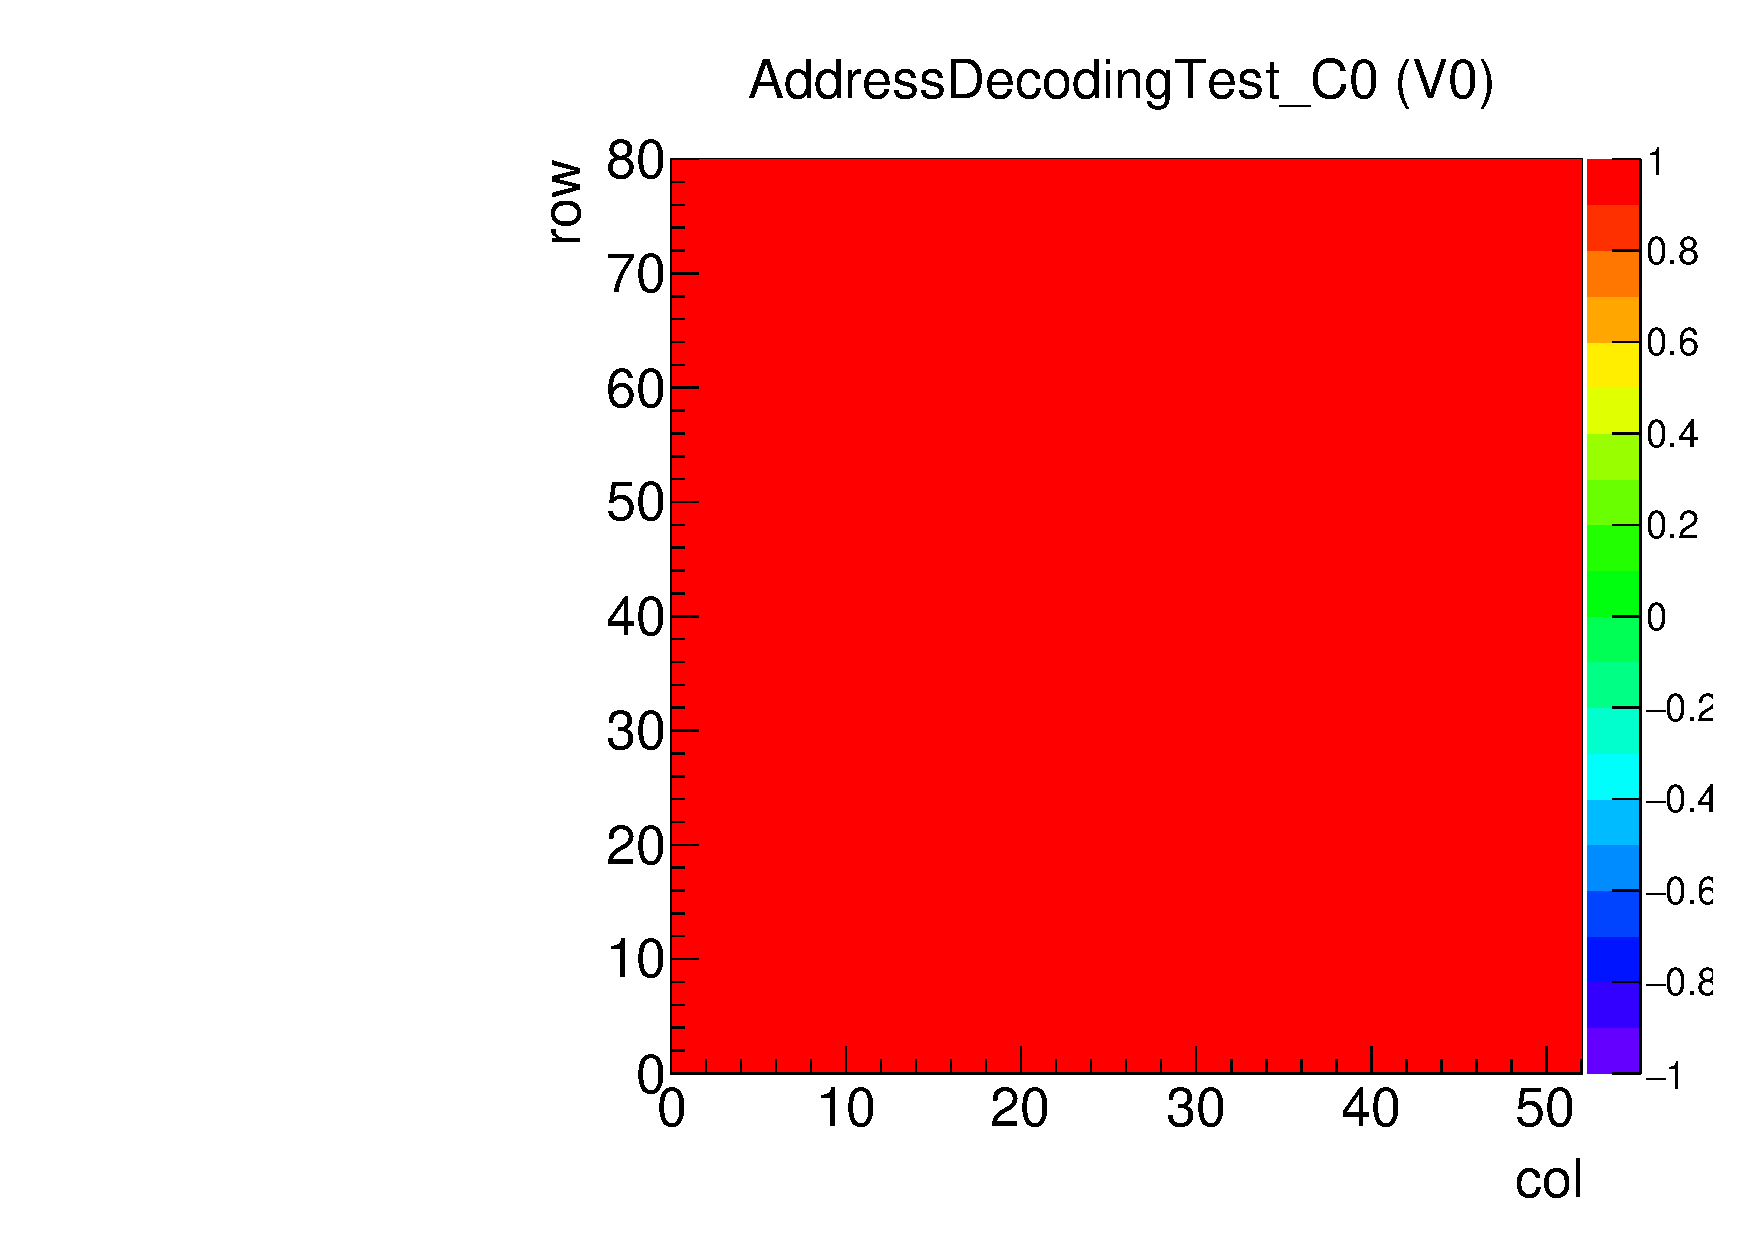
\includegraphics[width=1.0\textwidth]{figures/alive_AddressDecodingTest.pdf}
  \caption{Created by the {\tt AddressDecoding} test.
  1 (good), 0 (dead), -1 (mask problem).}
  \label{fig:alive_AddressDecodingTest}
\end{minipage}
\end{figure}
